\begin{definition}{Modèles de Markov}{markovmodel}
    Les \textbf{Modèles de Markov} sont une sorte de réseaux bayésiens qui décrivent 
    l'évolution d'un système dans le temps. Ils sont composés de variables 
    aléatoires $X_1, X_2, \dots, X_n$ qui représentent l'état du système à 
    différents moments dans le temps. Les variables aléatoires sont liées par 
    des probabilités de transition $P(X_t | X_{t-1})$ qui décrivent la 
    probabilité de passer d'un état à l'autre, comment l'état 
    du système évolue dans le temps.
\end{definition}

Ces modèles sont utiles pour prédire l'état d'un système à un moment donné. 

% Ils doivent cependant respecter la propriété de Markov, qui stipule que 
% l'état du système à un moment donné ne dépend que de l'état précédent.

\begin{theorem}{Processus Markovien}{markov}
    Soit $X_1, X_2, \dots, X_n$ une séquence de variables aléatoires. 
    Si la propriété de Markov est respectée, alors 
    \begin{align*}
        P(X_t | X_{t-1}, X_{t-2}, \dots, X_1) = P(X_t | X_{t-1})
    \end{align*}
    Cela signifie que \textbf{le future} est \textbf{indépendant }du \textbf{passé}, étant 
    donné le \textbf{présent}.
\end{theorem}

\begin{theorem}{Proccessus Stationnaire}{stationnaire}
    Soit $X_1, X_2, \dots, X_n$ une séquence de variables aléatoires. 
    Si la propriété de Markov est respectée, alors 
    \begin{align*}
        P(X_t | X_{t-1}) = P(X_{t+1} | X_t)
    \end{align*}
    Cela signifie que la probabilité de transition est la même pour tous les instants. 
    On dit que le modèle est \textbf{stationnaire}. 
\end{theorem}

\begin{remark}\leavevmode
    Lorsque l'instant $t$ est indépendant des instants $t-2, t-3, \dots, 1$, sachant $t-1$,
    on dit que le modèle est d'ordre 1. 
    Il este possible d'avoir des modèles d'ordre supérieur, dans lequel l'instant $t$ dépends 
    des $k$ instants précédents.
\end{remark}

Pour calculer la probabilité de distribution conjointe d'un modèle de Markov, 
il faut utiliser la propriété de Markov et la règle de la chaîne. 
\begin{align*}
    P(X_1, X_2, \dots, X_n) &= P(X_1) P(X_2 | X_1) P(X_3 | X_2, X_1) \dots P(X_n | X_{n-1}, \dots, X_1) \\
                            &= P(X_1) \prod_{t=2}^n P(X_t | X_{t-1}) 
\end{align*}

\subsection{Le modele qu'on ne trouve pas} % (fold)
\label{sub:le_modele_qu_on_ne_trouve_pas}

La différence avec un modèle de Markov, c'est que un modèle de Markov caché est un modèle 
dans lequel après chaque état, une observation est générée. On peut alors 
utiliser les observations pour inférer l'état du système.

Nous supposons également que l'observation est générée \textbf{uniquement par } l'état courant du système.
\begin{align*}
    P(E_t | X_{1:t}, E_{1:t-1} ) = P(E_t | X_t) 
\end{align*}
Sachant que l'état du système est connu, l'observation est indépendante des observations précédentes 
ainsi que des états précédents.

\begin{example}\leavevmode
    Un gardien de sécurité passe un mois dans un édifice sous-terrain, sans sortir. Chaque
    jour, son directeur arrive avec ou sans parapluie. Le gardien veut inférer la possibilite
    qu'il ait plu ou non en fonction de la sequence des observations du parapluie.

    Voici le modèle de Markov pour ce problème. 
    \begin{itemize}
        \item \textbf{Variables}: $X_t$= {$R_t$} qui représentre \textit{Rain} et $E_t = {U_t}$ qui représente \textit{Umbrella}.
        \item Dépendances entre les variables, càd Modèle de Markov:
            \begin{figure}[H]
                \centering
                \scalebox{0.8}{
                    \begin{minipage}{0.45\textwidth}
                        \begin{tikzpicture}
                              % Dessinez les nœuds du graphe
                            \node[state] (0) at (0,0) {$Rain_{t-1}$};
                            \node[state] (1) [right =of 0] {$Rain_t$}; 
                            \node[state] (4) [right =of 1] {$Rain_{t+1}$}; 
                            \node[state] (2) [below =of 0] {$Umbrella_{t-1}$}; 
                            \node[state] (3) [right =of 2] {$Umbrella_t$}; 
                            \node[state] (5) [right =of 3] {$Umbrella_{t+1}$};

                            \path (0) edge[arrow] (1); 
                            \path (1) edge[arrow] (4); 
                            \path (0) edge[arrow] (2);
                            \path (1) edge[arrow] (3);
                            \path (4) edge[arrow] (5);
                        \end{tikzpicture}
                        \caption{Modèle de Markov}
                        \label{fig:ex1}
                    \end{minipage}
                }
            \end{figure}
        \item Modèle de transitions: $P(R_t | R_{t-1})$ et $P(U_t | R_t)$ \textit{Stationnaire}
    \end{itemize}
    Nous voyons bien que l'état du système à un moment donné ne dépend que de l'état précédent. 
    Et que les observations sont générées uniquement par l'état courant du système.

\end{example}


Pour calculuer la probabilité de distribution conjointe d'un modèle de Markov caché, 
il faut utiliser la propriété de Markov et la règle de la chaîne. 
\begin{align*}
    P(X_1, X_2, \dots, X_n, E_n) &= P(X_1) P(X_2 | X_1) P(X_3 | X_2, X_1) \dots P(X_n | X_{n-1}, \dots, X_1) P(E_n | X_n) \\
                            &= P(X_1) \prod_{t=2}^n P(X_t | X_{t-1}) P(E_t | X_t)
\end{align*}

% subsection Celui qu'on ne trouve pas (end)

\subsection{Inférence} % (fold)
\label{sub:inference}

Il y a plusieurs problèmes d'inférence que l'on peut résoudre avec les modèles de Markov cachés. 

\begin{itemize}
    \item \textbf{Filtering}: Calculer la distribution de probabilité de l'état courant du système, 
    sachant toutes les observations jusqu'à maintenant. 
    \begin{align*}
        P(X_t | E_{1:t}) 
    \end{align*}
    \item \textbf{Prediction}: Calculer la distribution de probabilité de l'état futur du système, 
    sachant toutes les observations jusqu'à maintenant. Sans tenir compte des observations futures.
    \begin{align*}
        P(X_{t+k} | E_{1:t}) 
    \end{align*}
    \item \textbf{Smoothing}: Calculer la distribution de probabilité de l'état passé du système, 
    sachant toutes les observations jusqu'à maintenant. Meilleure estimation de l'état passé. \textit{Learning}
    \begin{align*}
        P(X_{t-k} | E_{1:t}) 
    \end{align*}
    \item \textbf{Most Likely Explanation}: Calculer la séquence d'états \textbf{la plus probable}, 
    sachant toutes les observations jusqu'à maintenant. 
    \begin{align*}
        \arg \max_{X_{1:t}} P(X_{1:t} | E_{1:t}) = \arg \max_{X_{1:t}} P(X_{1:t} ,E_{1:t}) / P(E_{1:t}) = \arg \max_{X_{1:t}} P(X_{1:t} ,E_{1:t})
    \end{align*}
\end{itemize} 

\begin{figure}[H]
\begin{center}
        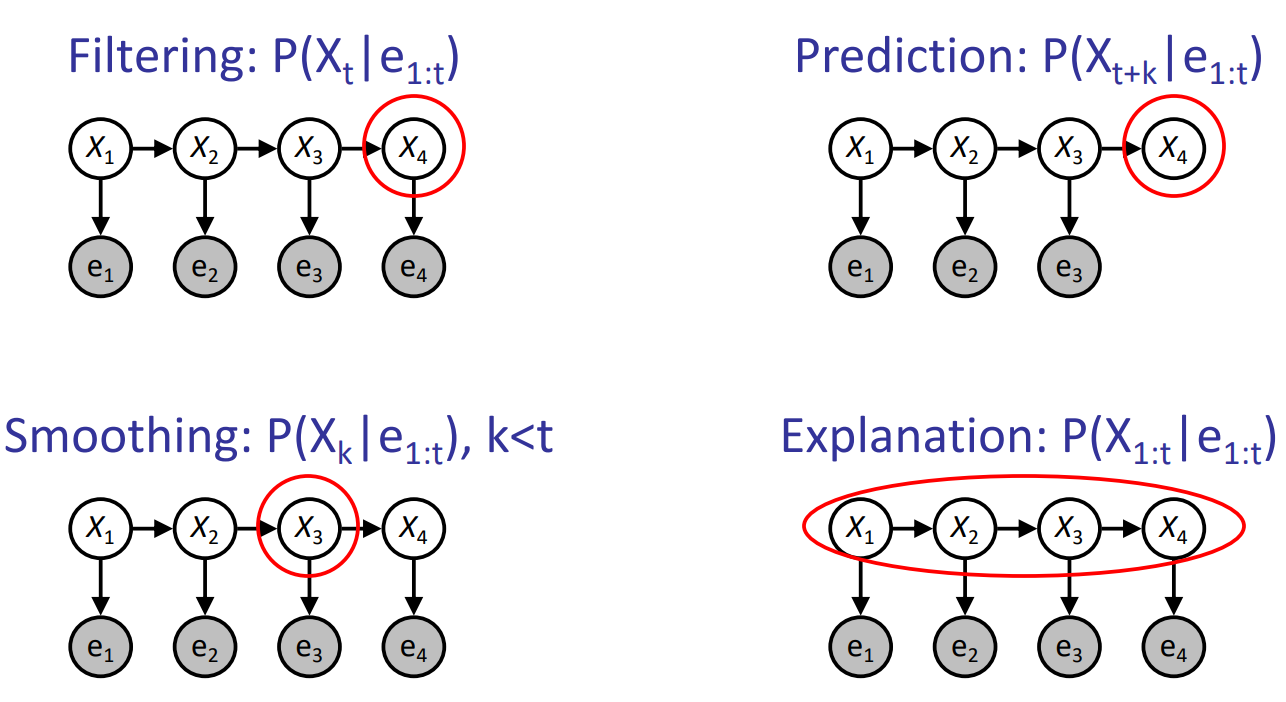
\includegraphics[width=0.37\textwidth]{../pictures/inferencehmm.png}
    \end{center}
    \caption{Inférence dans un modèle de Markov}\label{fig:inferencehmm}
\end{figure}

% subsection Inference (end)

\subsection{Chaines de Markov} % (fold)
\label{sub:chaines_de_markov}

Les chaines de Markov sont un cas particulier des modèles de Markov. 
Elles sont composées d'un ensemble d'états $S = {s_1, s_2, \dots, s_n}$ et d'une matrice de transition 
$T$ qui décrit la probabilité de passer d'un état à l'autre.
\begin{align*}
    T_{ij} = P(X_t = s_j | X_{t-1} = s_i) 
\end{align*} 
(même définition que pour les modèles de Markov, c'est juste moins général)




% subsection Chaines de Markov (end)



